\documentclass[
11pt, % The default document font size, options: 10pt, 11pt, 12pt
%codirector, % Uncomment to add a codirector to the title page
]{charter} 


% El títulos de la memoria, se usa en la carátula y se puede usar el cualquier lugar del documento con el comando \ttitle
\titulo{Modelo de inteligencia artificial para la regulación de temperatura en equipos de inducción de hipotermia} 

% Nombre del posgrado, se usa en la carátula y se puede usar el cualquier lugar del documento con el comando \degreename
\posgrado{Carrera de Especialización en Inteligencia Artificial} 
%\posgrado{Carrera de Especialización en Internet de las Cosas} 
%\posgrado{Carrera de Especialización en Inteligencia Artificial}
%\posgrado{Maestría en Sistemas Embebidos} 
%\posgrado{Maestría en Internet de las cosas}
% IMPORTANTE: no omitir titulaciones ni tildación en los nombres, también se recomienda escribir los nombres completos (tal cual los tienen en su documento)
% Tu nombre, se puede usar el cualquier lugar del documento con el comando \authorname
\autor{Ing. Ezequiel Fernandez}

% El nombre del director y co-director, se puede usar el cualquier lugar del documento con el comando \supname y \cosupname y \pertesupname y \pertecosupname
\director{Dr. Ing. Tobías Canavesi}
\pertenenciaDirector{FIUBA} 

\codirector{} % para que aparezca en la portada se debe descomentar la opción codirector en los parámetros de documentclass
\pertenenciaCoDirector{}

% Nombre del cliente, quien va a aprobar los resultados del proyecto, se puede usar con el comando \clientename y \empclientename
\cliente{Marcelo Castiglione}
\empresaCliente{AmrrA Electromedicina}
 
\fechaINICIO{23 de abril de 2024}		%Fecha de inicio de la cursada de GdP \fechaInicioName
\fechaFINALPlan{11 de junio de 2024} 	%Fecha de final de cursada de GdP
\fechaFINALTrabajo{9 de diciembre de 2024}	%Fecha de defensa pública del trabajo final


\begin{document}

\maketitle
\thispagestyle{empty}
\pagebreak


\thispagestyle{empty}
{\setlength{\parskip}{0pt}
\tableofcontents{}
}
\pagebreak


\section*{Registros de cambios}
\label{sec:registro}


\begin{table}[ht]
\label{tab:registro}
\centering
\begin{tabularx}{\linewidth}{@{}|c|X|c|@{}}
\hline
\rowcolor[HTML]{C0C0C0} 
Revisión & \multicolumn{1}{c|}{\cellcolor[HTML]{C0C0C0}Detalles de los cambios realizados} & Fecha      \\ \hline
0      & Creación del documento    &\fechaInicioName \\ \hline
1      & Se completa hasta el punto 5 inclusive   & 7  de mayo de 2024 \\ \hline
2      & Se completa hasta el punto 9 inclusive  & 14  de mayo de 2024 \\ \hline
3      & Se completa hasta el punto 12 inclusive                & 21 de mayo de 2024 \\ \hline
4      & Se completa el plan	                                 & 28 de mayo de 2024 \\ \hline

% Si hay más correcciones pasada la versión 4 también se deben especificar acá

\end{tabularx}
\end{table}

\pagebreak



\section*{Acta de constitución del proyecto}
\label{sec:acta}

\begin{flushright}
Buenos Aires, \fechaInicioName
\end{flushright}

\vspace{2cm}

Por medio de la presente se acuerda con el \authorname\hspace{1px} que su Trabajo Final de la \degreename\hspace{1px} se titulará ``\ttitle'' y consistirá en la implementación de un modelo de inteligencia artificial prototipo para optimizar el rendimiento de un sistema de regulación de temperatura para uso en tratamientos de de pacientes neonatales con hipoxia. Además se analizará la incidencia de los distintos atributos en la predicción. El trabajo tendrá un presupuesto preliminar estimado de 600 horas y un costo estimado de \$ 57.645.000, con fecha de inicio el \fechaInicioName\hspace{1px} y fecha de presentación pública el \fechaFinalName.

Se adjunta a esta acta la planificación inicial.

\vfill

% Esta parte se construye sola con la información que hayan cargado en el preámbulo del documento y no debe modificarla
\begin{table}[ht]
\centering
\begin{tabular}{ccc}
\begin{tabular}[c]{@{}c@{}}Dr. Ing. Ariel Lutenberg \\ Director posgrado FIUBA\end{tabular} & \hspace{2cm} & \begin{tabular}[c]{@{}c@{}}\clientename \\ \empclientename \end{tabular} \vspace{2.5cm} \\ 
\multicolumn{3}{c}{\begin{tabular}[c]{@{}c@{}} \supname \\ Director del Trabajo Final\end{tabular}} \vspace{2.5cm} \\
\end{tabular}
\end{table}




\section{1. Descripción técnica-conceptual del proyecto a realizar}
\label{sec:descripcion}

El objetivo de este proyecto será contar con un modelo de inteligencia artificial prototipo que estime la temperatura del agua que circula en un equipo utilizado para la inducción de hipotermia a pacientes neonatales. Además se hará foco en la incidencia de los parámetros que se disponen en el cálculo para aportar al conocimiento sobre estos tratamientos. Esto puede significar a futuro una mejora en un producto que desarrolla la empresa y brindar a quienes necesiten este tratamiento un desarrollo superador del mismo respecto a la actualidad. El proyecto será desarrollado dentro del marco del programa de vinculación. 

La empresa es AmrrA y los equipos en cuestión tienen el nombre Amrraterm HTF. Estos sistemas se utilizan con el propósito de inducir una hipotermia controlada en pacientes neonatales. Existen contextos en los cuales esto proporciona una mejor evolución de los pacientes. El principal caso de uso es el de pacientes que sufren hipoxia al nacer, esto es, falta de oxígeno en el cerebro. En estos casos, a temperatura corporal normal la interacción entre las neuronas es alta y se pueden desarrollar efectos adversos en la capacidad cerebral del paciente. Por esto un tratamiento estándar es el de inducir hipotermia por 72 horas a fin de minimizar los efectos que la hipoxia puede generar a futuro en los pacientes. 

Para lograr esto el procedimiento estándar es sedar al paciente y colocarlo dentro de una incubadora, donde es envuelto en las mantas que forman parte del equipo. Por estas mantas circula agua destilada. El equipo recibe como dato de entrada la temperatura objetivo a la cual se quiere llevar al paciente, que suele ser de 33,5º C, y regula la temperatura del agua en función de la temperatura objetivo y la actual del paciente. Una vez terminado el tratamiento de hipotermia, el equipo funciona en un modo llamado rampa, en el cual sube paulatinamente la temperatura hasta llegar a un estado normal.

Si bien existe un protocolo, que es el antes descrito, se dan ocasiones en las que se hace un mal uso del equipo, estableciendo como temperatura objetivo un valor inferior a los 33,5º C o utilizándolo en pacientes que no están correctamente sedados en la incubadora. Estos casos podrían afectar los resultados del modelo por lo que deberían categorizarse.

En la actualidad la temperatura del agua es regulada por un algoritmo de lógica difusa. En un rango de pesos estándar de los pacientes (entre 2,5 kg y 3,5 kg) el algoritmo funciona correctamente, pero es posible que en pesos inferiores o superiores haya comportamientos que este proyecto pueda mejorar. Se desarrollará este modelo para evaluar si funciona mejor que el algoritmo actual en ese rango, en los valores inferiores o en los superiores de peso. 

Se utilizarán diversos datos para construir un modelo acorde al problema como el peso del paciente, la edad, la temperatura objetivo y las variaciones de temperatura del agua y paciente. Además de construir un modelo superador, también se busca detectar la incidencia de ciertos parámetros, como el peso del paciente, que no se utiliza por el algoritmo actual. Para evaluar el comportamiento del modelo se debe implementar un entorno, en algún lenguaje de programación a conveniencia de las partes, que permita evaluar y comparar resultados. 

En la figura \ref{fig:diagBloquesActual} se presenta un diagrama del funcionamiento del equipo actualmente. La temperatura del agua es regulada a través de un sistema térmico. Periódicamente un algoritmo de lógica difusa calcula la temperatura que debe tener el agua en el siguiente periodo.

\begin{figure}[htpb]
	\centering 
	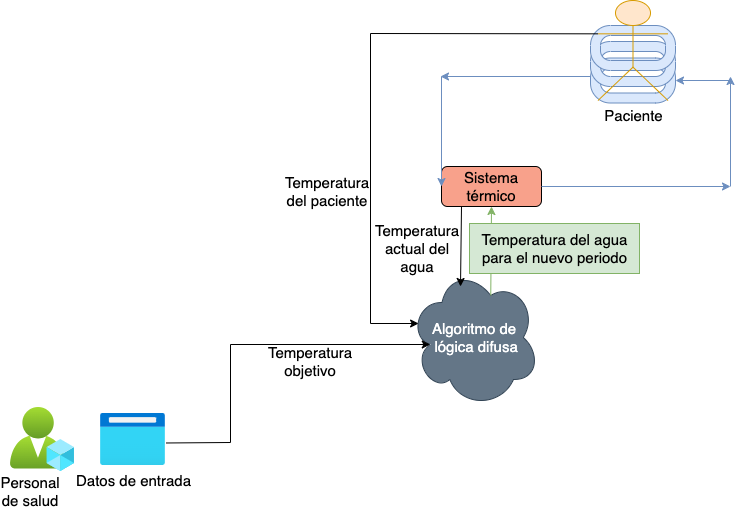
\includegraphics[width=.95\textwidth]{./Figuras/amrra-diagrama1.png}
	\caption{Diagrama en bloques del sistema actual.}
	\label{fig:diagBloquesActual}
\end{figure}

En la figura  \ref{fig:diagBloquesFuturo} se puede ver la incorporación de un modelo de inteligencia artificial en comparación con el actual.

\begin{figure}[htpb]
	\centering 
	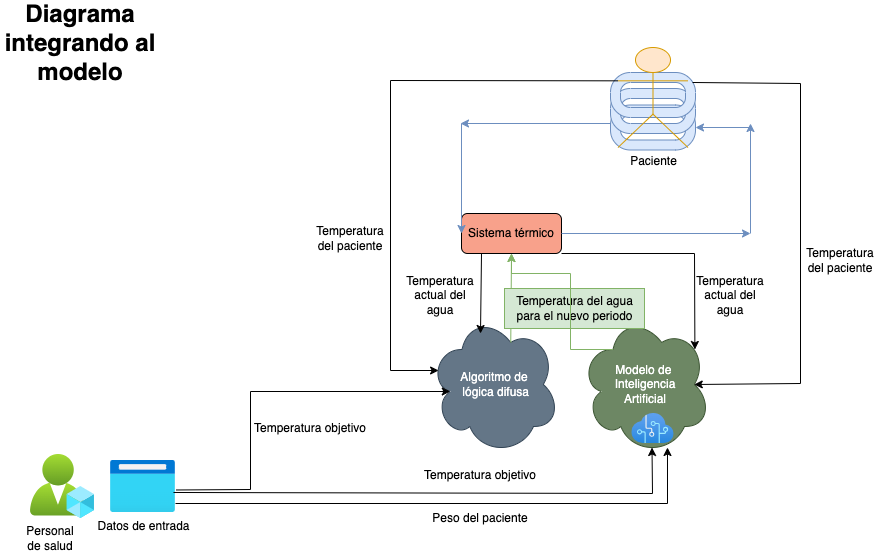
\includegraphics[width=.95\textwidth]{./Figuras/amrra-diagrama2.png}
	\caption{Diagrama en bloques del sistema integrando al modelo.}
	\label{fig:diagBloquesFuturo}
\end{figure}

Si bien existen artículos en la actualidad que analizan el uso de diversos modelos de \textit{machine learning} en contextos de hipotermia, la mayoría ponen el foco en estimar la mortalidad de los casos o en predecir potenciales casos de hipotermia. Estos enfoques son interesantes para evaluar los riesgos de someter al paciente bajo este tratamiento pero no son el objetivo de este proyecto. En este caso el foco estará en un modelo que regule de forma óptima la inducción a hipotermia de un paciente.

El presente proyecto se ve impulsado por buscar innovación con el uso tecnologías nuevas en un producto clave de la empresa. Se evaluará si esto resulta en una mejora en la calidad del producto y por esto en los tratamientos de los pacientes. Además se analizará la incidencia del peso y demás datos en el tratamiento para la correcta inducción de hipotermia, lo que aporta al conocimiento que se tiene actualmente sobre estos tratamientos. 

A futuro se llevará a cabo la integración del modelo resultante al sistema embebido del producto comercial Amrraterm HTF.

\section{2. Identificación y análisis de los interesados}
\label{sec:interesados}

\begin{table}[ht]
%\caption{Identificación de los interesados}
%\label{tab:interesados}
\begin{tabularx}{\linewidth}{@{}|l|X|X|l|@{}}
\hline
\rowcolor[HTML]{C0C0C0} 
Rol           & Nombre y Apellido & Organización 	& Puesto 	\\ \hline
Auspiciante   & Área de Ingeniería  &  AmrrA electromedicina &        Área de Ingeniería	\\ \hline
Cliente       &  Área de Ingeniería      & AmrrA electromedicina		&        Área de Ingeniería	\\ \hline
Impulsor      &  Marcelo  Castiglione &  AmrrA electromedicina	&        Área de Ingeniería	\\ \hline
Responsable   & \authorname       & FIUBA        	& Alumno 	\\ \hline
Colaboradores &  Ing. Laneri                 &      AmrrA electromedicina        	&   Área de Ingeniería	\\ \hline
Orientador    & \supname	      & \pertesupname 	& Director del Trabajo Final \\ \hline
Usuario final &   Médicos    &    Hospitales	&        -	\\ \hline
\end{tabularx}
\end{table}
 
\begin{itemize}
	\item Orientador: el director del trabajo es experto en la temática y va a ayudar con la exploración inicial y definición de estrategias para llegar a los objetivos.
	\item Impulsor: está muy interesado en el tema y en ayudar en lo que esté a su alcance.
	\item Usuario final: los médicos son quienes utilizarán los equipos y pueden  hacer comentarios acerca del uso de estos, pero también se debe mencionar a los pacientes que serán tratados.
\end{itemize}


\section{3. Propósito del proyecto}
\label{sec:proposito}
	
El propósito de este proyecto está orientado a cubrir los siguientes aspectos:
\begin{itemize}
	\item Desde un punto de vista funcional, consistirá en brindar un modelo de inteligencia artificial que estime cambio de temperatura óptimo para la salud del paciente en un instante.
	\item Desde un punto de vista conceptual, se desea analizar la incidencia del peso del paciente en este tratamiento.
	\item Desde un punto de vista personal, servirá como un medio formal para acreditar la Especialización en Inteligencia Artificial y como primer experiencia en un proyecto de esta temática en un ambiente cercano al laboral.	
\end{itemize}



\section{4. Alcance del proyecto}
\label{sec:alcance}

El alcance de este proyecto está orientado a desarrollar una solución de inteligencia artificial acorde al problema planteado. Se cubrirán los siguientes ejes de trabajo:

\begin{itemize}
	\item Entendimiento del problema y negocio: profundo aprendizaje sobre el contexto y rol que tendrá el modelo.
	\item Adquisición de datos y análisis de los mismos: análisis y preprocesamiento de los datos y generación de datos sintéticos en caso de escasez.
	\item Modelado: se evaluarán diversos modelos, buscando al de mejor rendimiento en función de poder predictivo y significado de los atributos.
	\item Resultado conceptual: se evaluará la incidencia de cada parámetro en las estimaciones del modelo.
	\item Visibilidad: se ofrecerá una forma de probar al modelo y de evaluarlo contra el algoritmo actual.
\end{itemize}

El presente proyecto no incluye: 
\begin{itemize}
	\item La incorporación del modelo a los equipos en funcionamiento.
	\item El despliegue del modelo en la nube.
	\item El desarrollo de una interfaz gráfica, una aplicación o una web.
\end{itemize}



\section{5. Supuestos del proyecto}
\label{sec:supuestos}

Para el desarrollo del presente proyecto se supone que: 

\begin{itemize}
	\item El desarrollo es alcanzable con los conocimientos actuales.
	\item El tiempo será suficiente para alcanzar los objetivos planteados. teniendo en cuenta imprevistos y cambios de enfoque posibles.
	\item Los accesos a la información y a los datos serán concedidos en tiempo y forma.
	\item La cantidad de datos disponibles y el preprocesamiento que pueda hacerse de los mismos será suficiente para un resultado aceptable.
\end{itemize}


\section{6. Requerimientos}
\label{sec:requerimientos}

\begin{enumerate}
	\item Requerimientos funcionales:
		\begin{enumerate}
			\item El modelo debe predecir el cambio de temperatura óptimo a aplicar.
			\item La salida del modelo debe ser conceptualmente análoga a la del algoritmo de lógica difusa utilizado actualmente, a fin de poder compararlos.
			\item El modelo debe dar una respuesta en un tiempo promedio menor o igual a 10 veces el tiempo promedio de respuesta del algoritmo actual.
			\item El sistema debe permitir ingresar datos de forma manual y mostrar el resultado.
			\item Se debe calcular la incidencia del peso y de los demás atributos en la solución.
		\end{enumerate}
	\item Requerimientos conceptuales:
		\begin{enumerate}
			\item Deben utilizarse datos sintéticos en el entrenamiento.
		\end{enumerate}
	\item Requerimiento de testing:
		\begin{enumerate}
			\item Se deben ejecutar pruebas secuenciales con datos reales y mostrar una comparación entre los resultados del modelo a implementar y del algoritmo actual.
			\item Se deben comparar tiempos entre el modelo propuesto y el algoritmo actual.
			\item Se debe calcular una métrica a definir para calcular la performance del modelo.
		\end{enumerate}
	\item Requerimiento de documentación:
		\begin{enumerate}
			\item Se deben documentar las decisiones tomadas.
			\item Se deben documentar los resultados de las pruebas y las distintas métricas.
			\item Se requiere documentar el código y las formas de utilizar al sistema.
		\end{enumerate}
	\item Requerimiento asociados con regulaciones
		\begin{enumerate}
			\item Se requiere que los casos utilizados no expongan datos que infrinjan derechos de privacidad.
		\end{enumerate}
\end{enumerate}

\section{7. Historias de usuarios (\textit{Product backlog})}
\label{sec:backlog}

En esta sección se describirán algunas historias de usuarios ponderadas en un sistema de puntos, según el rol de cliente.

Para determinar los puntos de cada historia se definen los siguientes criterios:
\begin{itemize}
	\item Cantidad de trabajo:
	\begin{itemize}
		\item Baja: 1 punto.
		\item Media: 3 puntos.
		\item Alta: 5 puntos.
	\end{itemize}
	\item Complejidad del trabajo:
		\begin{itemize}
			\item Baja: 2 puntos.
			\item Media: 5 puntos.
			\item Alta: 13 puntos.
		\end{itemize}
	\item Incertidumbre del trabajo:
		\begin{itemize}
			\item Baja: 3 puntos.
			\item Media: 5 puntos.
			\item Alta: 10 puntos.
		\end{itemize}
\end{itemize}

La cantidad de puntos de una historia de usuario estará definida por el número en la sucesión de Fibonacci mas cercano y mayor o igual a la suma del puntaje de los tres criterios definidos.

\begin{itemize}
	\item Como cliente, quiero contar con un modelo que estime el cambio de temperatura en el equipo para tratamientos de hipotermia.
		\begin{itemize}
			\item Cantidad de trabajo 5 puntos.
			\item Complejidad: 5 puntos.
			\item Incertidumbre: 10 puntos.
			\item Story Points: 5 + 5 + 10 = 20, tomando el siguiente de la sucesión de Fibonacci el puntaje es 21.
		\end{itemize}
	\item Como cliente, quiero conocer la incidencia del peso en el calculo de la variación de temperatura óptima para los pacientes.
		\begin{itemize}
			\item Cantidad de trabajo 1 punto.
			\item Complejidad: 5 puntos.
			\item Incertidumbre: 5 puntos.
			\item Story Points: 1 + 5 + 5 = 11, tomando el siguiente de la sucesión de Fibonacci el puntaje es 13.
		\end{itemize}
	\item Como cliente, quiero una guía que explique el funcionamiento y la forma de utilizar el modelo, a modo de integrarlo en el equipo en el futuro.
		\begin{itemize}
			\item Cantidad de trabajo 3 puntos.
			\item Complejidad: 2 puntos.
			\item Incertidumbre: 3 puntos.
			\item Story Points: 3 + 2 + 3 = 8, tomando el número mayor o igual mas cercano de la sucesión de Fibonacci el puntaje es 8.
		\end{itemize}
	\item Como cliente, quiero un entorno en el cual comparar el resultado del modelo y el del algoritmo actual para una entrada dada.
	\begin{itemize}
		\item Cantidad de trabajo 3 puntos.
		\item Complejidad: 2 puntos.
		\item Incertidumbre: 3 puntos.
		\item Story Points: 3 + 2 + 3 = 8, tomando el número mayor o igual mas cercano de la sucesión de Fibonacci el puntaje es 8.
	\end{itemize}
\end{itemize}

\section{8. Entregables principales del proyecto}
\label{sec:entregables}

Los entregables del proyecto son:

\begin{itemize}
	\item Manual de uso e integración del sistema.
	\item Código fuente.
	\item Diagrama de funcionamiento del sistema.
	\item Informe de pruebas.
	\item Memoria del trabajo final.
\end{itemize}

\section{9. Desglose del trabajo en tareas}
\label{sec:wbs}

\begin{enumerate}
\item Planificación general del proyecto (50 h).
	\begin{enumerate}
	\item Redacción de la descripción técnica y propósito (20 h).
	\item Definición del alcance, riesgos y requerimientos (10 h).
	\item Planificación del desarrollo (20 h).
	\end{enumerate}
\item Exploración y preprocesamiento de datos (110 h).
	\begin{enumerate}
	\item Análisis exploratorio de los datos (10 h).
	\item Generación de datos sintéticos (40 h).
	\item Preprocesamiento y categorización de datos (40 h).
	\item Etiquetado de datos según contextos de uso (20 h).
	\end{enumerate}
\item Desarrollo del modelo (230 h).
	\begin{enumerate}
	\item Definición del criterio de medición y comparación de modelos (16 h).
	\item Selección de modelos a utilizar (16 h).
	\item Implementación de los modelos (40 h).
	\item Experimentación con los modelos (40 h).
	\item Comparación de resultados y elección de modelo a utilizar (8 h).	
	\item Optimización del modelo elegido (40 h).
	\item Refinamiento del modelo y entendimiento del comportamiento del mismo (40 h).
	\item Cálculo de la incidencia de los parámetros en la predicción (30 h).
	\end{enumerate}
\item Desarrollo del entorno donde se prueba el modelo (68 h).
\begin{enumerate}
	\item Definición del lenguaje (8 h).
	\item Desarrollo del entorno (30 h).
	\item Integración del entorno con los algoritmos a probar (30 h).
\end{enumerate}
\item Evaluación y pruebas comparativas (72 h).
	\begin{enumerate}
	\item Pruebas comparativas con el algoritmo actual (24 h).
	\item Generación de gráficos y documentación de pruebas (16 h).
	\item Análisis de resultados (16 h).
	\item Comparación de tiempos de respuesta de los algoritmos (16 h).
	\end{enumerate}
\item Elaboración de la memoria (80 h).
	\begin{enumerate}
	\item Escritura de la memoria del trabajo final (40 h).
	\item Elaboración de la presentación para la exposición final (20 h).
	\item Escritura de la documentación técnica del modelo y su uso para el cliente (20 h).
	\end{enumerate}
\end{enumerate}

Cantidad total de horas: 610 h.

\section{10. Diagrama de Activity On Node}
\label{sec:AoN}

En la figura \ref{fig:aon} se puede ver un diagrama Activity on Node del proyecto, donde las unidades de tiempo están expresadas en horas, y en la figura \ref{fig:aon_referencias} se ven las referencias del diagrama.

\begin{figure}[htpb]
	\centering 
	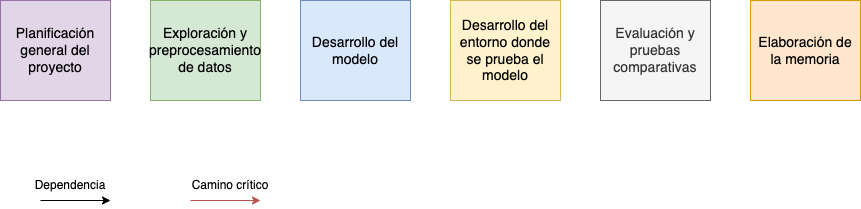
\includegraphics[width=1.05\textwidth]{./Figuras/amrra-aon-referencias.png}
	\caption{Referencias del diagrama Activity on Node.}
	\label{fig:aon_referencias}
\end{figure}

\begin{figure}[htpb]
	\centering 
	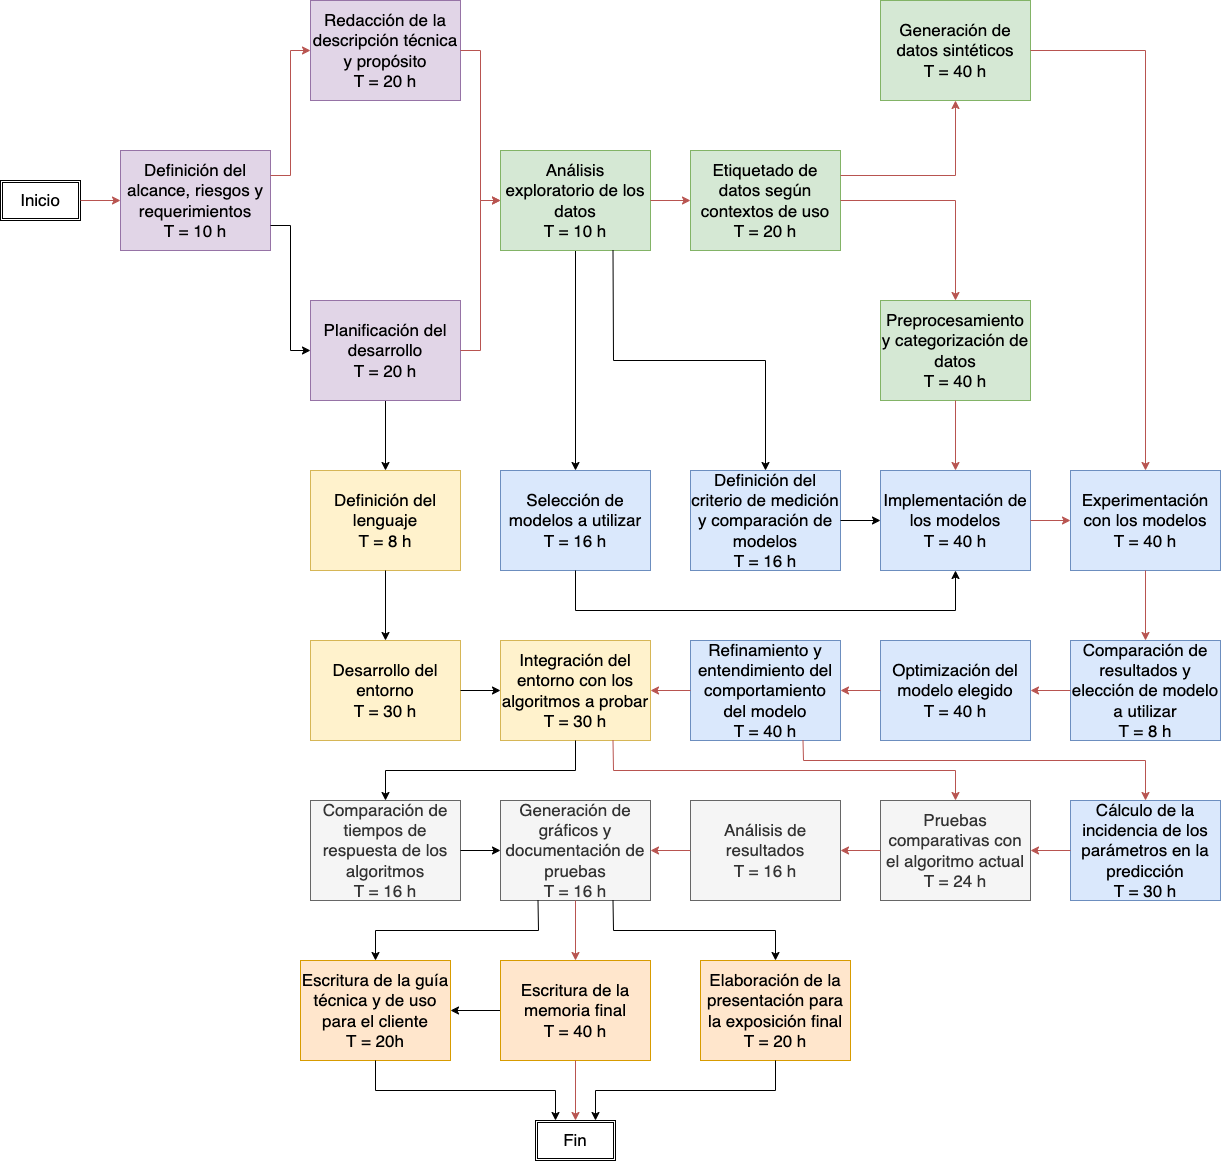
\includegraphics[width=1\textwidth]{./Figuras/amrra-AON.png}
	\caption{Activity on Node del proyecto.}
	\label{fig:aon}
\end{figure}

\section{11. Diagrama de Gantt}
\label{sec:gantt}

A continuación se muestra el diagrama de Gantt del proyecto, dividido en dos partes.

En la figura \ref{fig:gantt_tareas} se muestra el listado de tareas definido previamente, y en la figura  \ref{fig:gantt_diagram} se ve el diagrama. Las fechas se muestran en inglés debido al software utilizado. 

	\begin{figure}[htpb]
		\centering 
		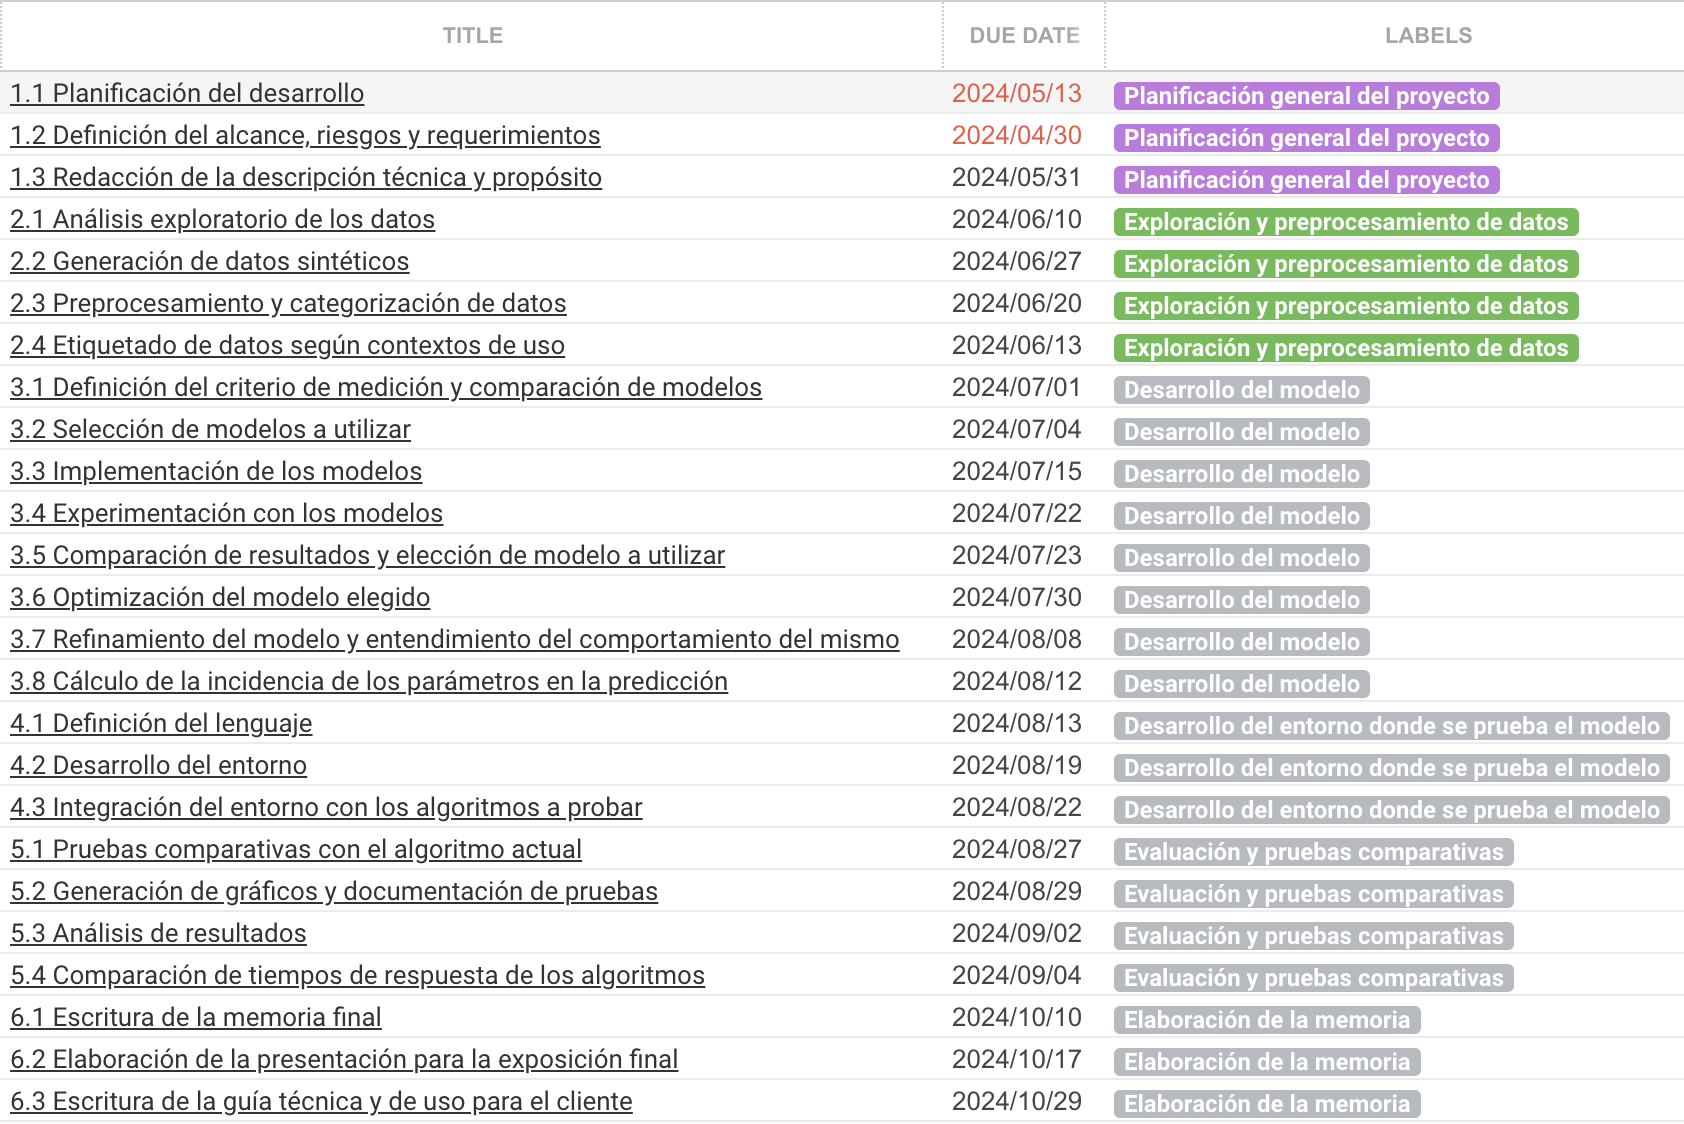
\includegraphics[height=.45\textheight]{./Figuras/gantt_tareas.png}
		\caption{Tareas del diagrama de Gantt.} %Modificar este título acorde.
		\label{fig:gantt_tareas}
	\end{figure}

\begin{landscape}
	\begin{figure}[htpb]
		\centering 
		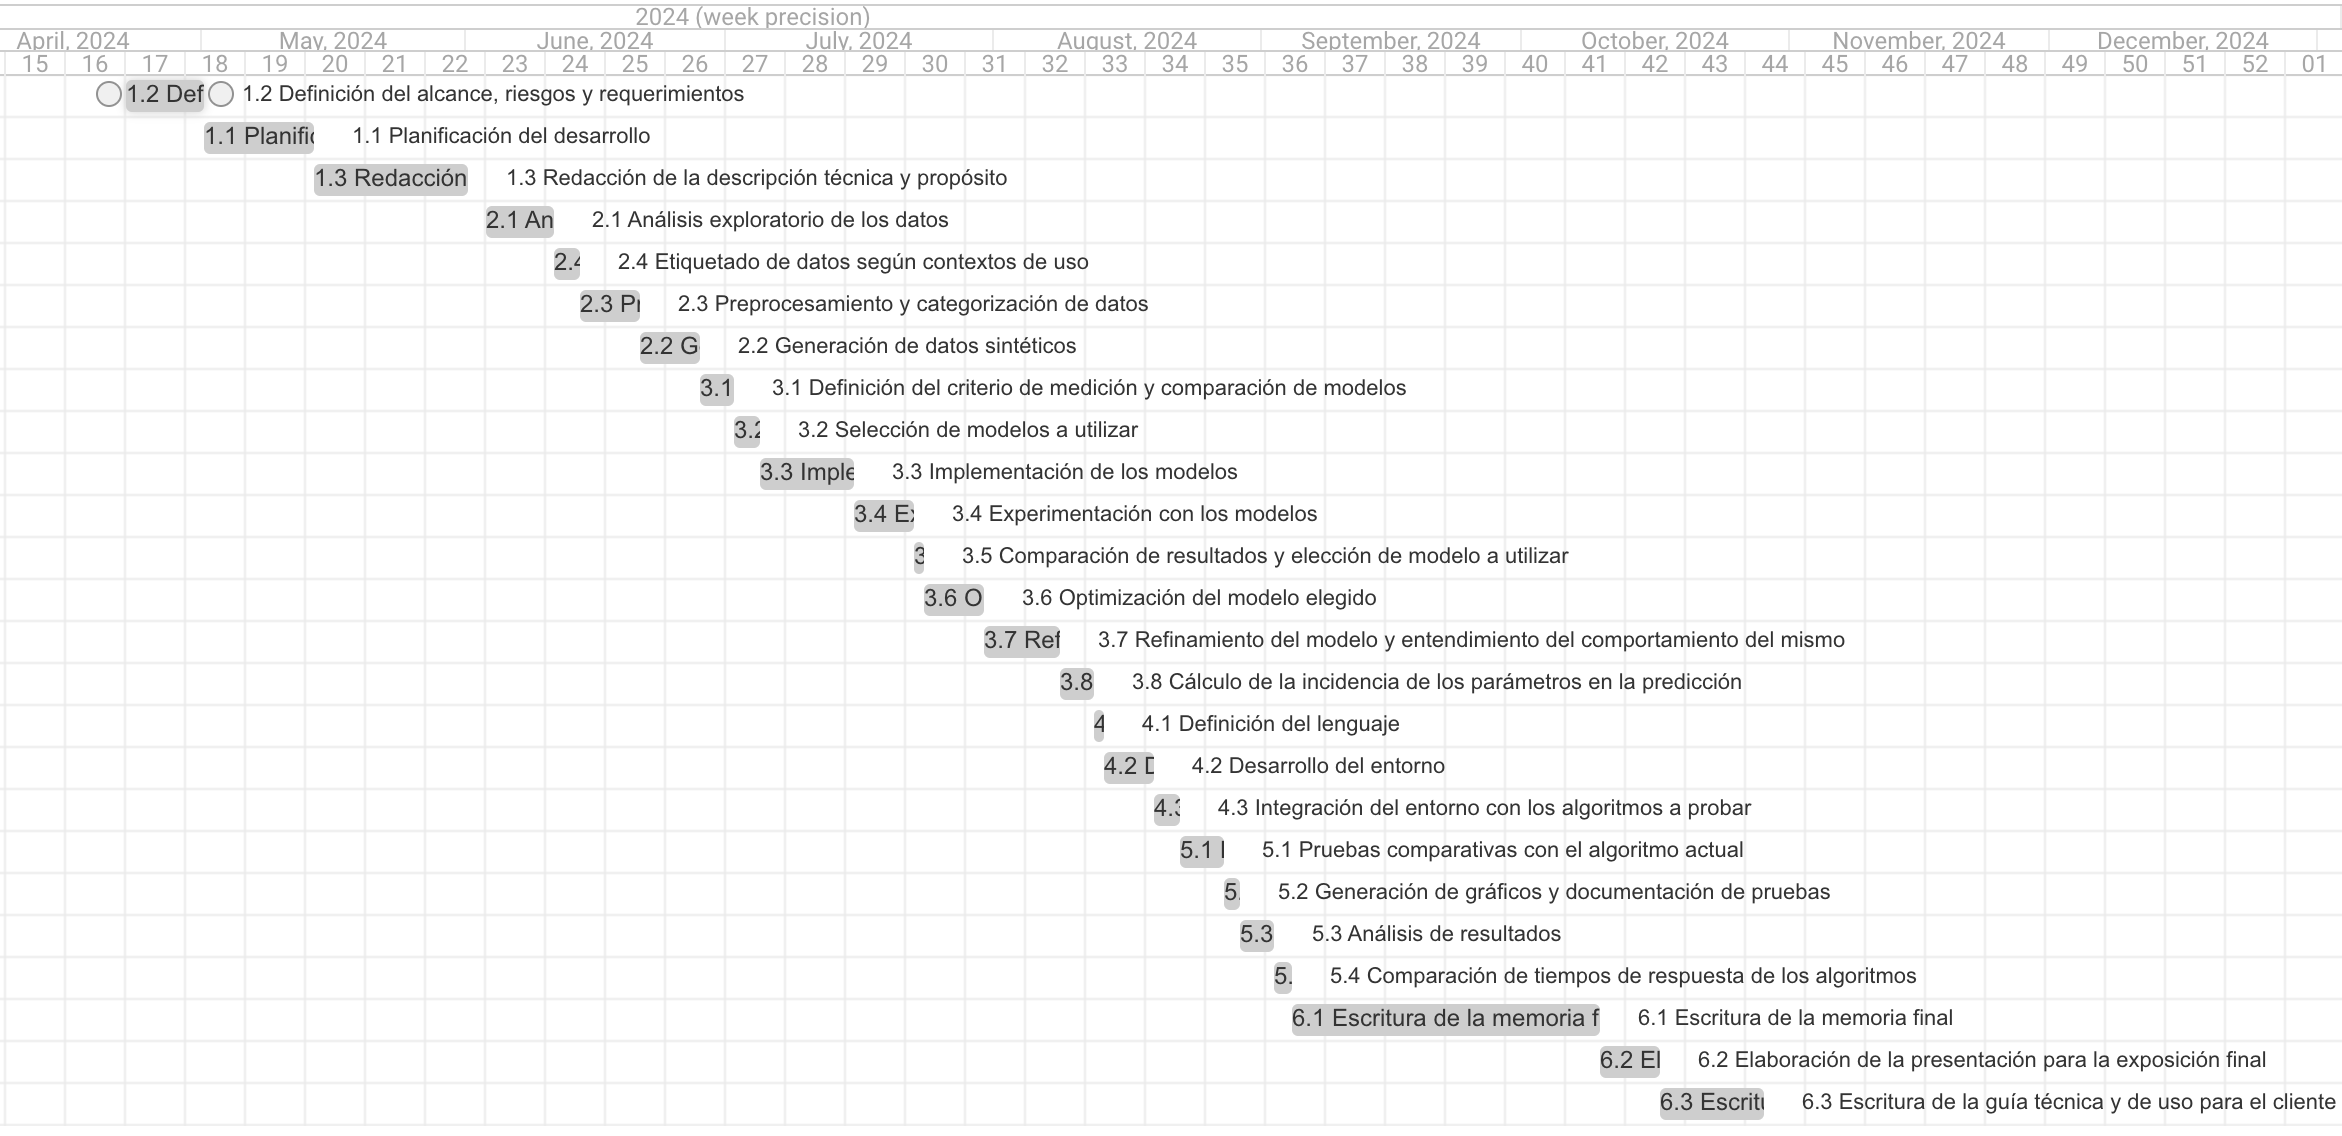
\includegraphics[height=.75\textheight]{./Figuras/gantt_complete.png}
		\caption{Diagrama de Gantt.} %Modificar este título acorde.
		\label{fig:gantt_diagram}
	\end{figure}
\end{landscape}

\section{12. Presupuesto detallado del proyecto}
\label{sec:presupuesto}

A continuación se detalla el presupuesto del proyecto, discriminado en costos directos e indirectos, expresado en pesos argentinos.

\begin{table}[htpb]
\centering
\begin{tabularx}{\linewidth}{@{}|X|c|r|r|@{}}
\hline
\rowcolor[HTML]{C0C0C0} 
\multicolumn{4}{|c|}{\cellcolor[HTML]{C0C0C0}COSTOS DIRECTOS} \\ \hline
\rowcolor[HTML]{C0C0C0} 
Descripción &
  \multicolumn{1}{c|}{\cellcolor[HTML]{C0C0C0}Cantidad} &
  \multicolumn{1}{c|}{\cellcolor[HTML]{C0C0C0}Valor unitario} &
  \multicolumn{1}{c|}{\cellcolor[HTML]{C0C0C0}Valor total} \\ \hline
 Horas de ingeniería &
  \multicolumn{1}{c|}{610 h} &
  \multicolumn{1}{c|}{\$ 67.500 } &
  \multicolumn{1}{c|}{\$ 41.175.000 } \\ \hline
\multicolumn{3}{|c|}{SUBTOTAL} &
  \multicolumn{1}{c|}{\$ 41.175.000 } \\ \hline
\rowcolor[HTML]{C0C0C0} 
\multicolumn{4}{|c|}{\cellcolor[HTML]{C0C0C0}COSTOS INDIRECTOS} \\ \hline
\rowcolor[HTML]{C0C0C0} 
Descripción &
  \multicolumn{1}{c|}{\cellcolor[HTML]{C0C0C0}Cantidad} &
  \multicolumn{1}{c|}{\cellcolor[HTML]{C0C0C0}Valor unitario} &
  \multicolumn{1}{c|}{\cellcolor[HTML]{C0C0C0}Valor total} \\ \hline
  40\% del costo directo  &
	\multicolumn{1}{|l|}{1}&
	\multicolumn{1}{|l|}{\$ 16.470.000 }&
	\multicolumn{1}{|l|}{\$ 16.470.000 }
   \\ \hline
\multicolumn{3}{|c|}{SUBTOTAL} &
  \multicolumn{1}{c|}{\$ 16.470.000 } \\ \hline
\rowcolor[HTML]{C0C0C0}
\multicolumn{3}{|c|}{TOTAL} &
\$ 57.645.000
   \\ \hline
\end{tabularx}%
\end{table}


\section{13. Gestión de riesgos}
\label{sec:riesgos}

A continuación se describirán los riesgos potenciales que se pueden presentar en el desarrollo del proyecto y los planes de mitigación.

a) Identificación de los riesgos y estimación de sus consecuencias:
 
Riesgo 1: los datos tomados de casos donde no se cumplió el protocolo de uso afectan la correctitud del modelo.
\begin{itemize}
	\item Severidad (S): 5. 
	Este riesgo tiene una severidad media ya que puede afectar directamente en la correctitud del modelo desviando ligeramente la predicción correcta.
	\item Probabilidad de ocurrencia (O): 6. 
	La probabilidad de este riesgo es media ya que desde la empresa comentan que han detectado múltiples usos sin que se aplique correctamente el protocolo.
\end{itemize}

Riesgo 2: no se dispone de la suficiente cantidad de datos.
\begin{itemize}
	\item Severidad (S): 9. 
	Reduce la probabilidad de que el modelo funcione correctamente
	\item Ocurrencia (O): 2.
	La probabilidad es baja ya que inicialmente se analizó la viabilidad del proyecto, y según las charlas iniciales se dispone de una cantidad de datos prometedora. Sin embargo no es seguro que estos datos serán lo suficientemente representativos del problema.
\end{itemize}

Riesgo 3: el modelo tiene un tiempo de respuesta mayor al del algoritmo actual.
\begin{itemize}
	\item Severidad (S): 2.
	El modelo se ejecutará periódicamente, actualmente cada 15 minutos, y es éste su único uso. Por esto un aumento en los tiempos de respuesta no representa un problema mayor.
	\item Ocurrencia (O): 8. 
	La probabilidad de ocurrencia es alta dado que es muy probable que los modelos a utilizar requieran cálculos más complejos que el algoritmo actual.
\end{itemize}

Riesgo 4: el modelo no tiene un nivel de predicción superador.
\begin{itemize}
	\item Severidad (S): 4.
	Este riesgo no invalida al proyecto en sí y tampoco implica que la realización del mismo no le aporta valor a la empresa.
	\item Ocurrencia (O): 3.
	La probabilidad de ocurrencia es baja ya que hay enfoques que prometen buenos resultados.
\end{itemize}

Riesgo 5: el poder de cómputo para entrenar los modelos es escaso.
\begin{itemize}
	\item Severidad (S): 7.
	Este riesgo tiene una severidad media/alta ya que puede afectar directamente en la correctitud del modelo.
	\item Probabilidad de ocurrencia (O): 5.
		La probabilidad de este riesgo es media ya que se utilizará la misma computadora con la que se entrenaron los modelos realizados durante la carrera, y hasta ahora esto resulto suficiente, pero podría darse que no lo sea para el proyecto.
\end{itemize}

b) Tabla de gestión de riesgos:      (El RPN se calcula como RPN=SxO)

\begin{table}[htpb]
\centering
\begin{tabularx}{\linewidth}{@{}|X|c|c|c|c|c|c|@{}}
\hline
\rowcolor[HTML]{C0C0C0} 
Riesgo & S & O & RPN & S* & O* & RPN* \\ \hline
1. Los datos tomados de casos donde no se cumplió el protocolo afectan la correctitud del modelo. & 5  & 6  &   30  &  4  &  1  &   4   \\ \hline
2. No se dispone de la suficiente cantidad de datos. & 9  & 2  &  18   &  -  &  -  &  -    \\ \hline
3. El modelo tiene un tiempo de respuesta mayor al del algoritmo actual.& 2  & 8  &  16   &  -  &  -  &  -    \\ \hline
4. El modelo no tiene un nivel de predicción superador.&  4 & 3  &  12   &  -  &  -  &  -    \\ \hline
5. El poder de cómputo para entrenar los modelos es escaso.  & 7  & 5  &  35   &  7  &  1  &   7   \\ \hline
\end{tabularx}%
\end{table}

Criterio adoptado: 

Se tomarán medidas de mitigación en los riesgos cuyos números de RPN sean mayores a 25.

Nota: los valores marcados con (*) en la tabla corresponden luego de haber aplicado la mitigación.

c) Plan de mitigación de los riesgos que originalmente excedían el RPN máximo establecido:
 
Riesgo 1: Se categorizarán los datos según si se percibe que se cumplió el protocolo o no, y se utilizarán los datos obtenidos en un contexto donde se haya cumplido el protocolo. Se evaluará entrenar un modelo para casos donde no se cumpla el protocolo si la cantidad de datos es suficiente.
  Nueva asignación de S y O, con su respectiva justificación:
  \begin{itemize}
	\item Severidad (S*): 4.
          La severidad es media ya que los datos pueden afectar al modelo, pero seguramente sea en menor cantidad.
	\item Probabilidad de ocurrencia (O*): 1.
          Es altamente probable eliminar la mayoría de los datos que no representan correctamente al contexto.
	\end{itemize}

Riesgo 5: Se utilizará la plataforma Google Colaboratory para entrenar a algunos de los modelos. En caso de que esta plataforma no brinde el poder de cómputo suficiente en su versión gratuita se pagará una cuota para obtener el nivel de cómputo suficiente.
Nueva asignación de S y O, con su respectiva justificación:
\begin{itemize}
	\item Severidad (S*): 7.
	La severidad es medida/alta ya que esto puede afectar directamente la precisión del modelo.
	\item Probabilidad de ocurrencia (O*): 1.
	Es altamente probable que Google Colaboratory ofrezca el poder de cómputo que se necesita para este proyecto.
\end{itemize}

\section{14. Gestión de la calidad}
\label{sec:calidad}

A continuación se listan los requerimientos y las condiciones para su verificación y validación.

\begin{itemize} 
\item Req \#1: el modelo debe predecir el cambio de temperatura óptimo a aplicar.

\begin{itemize}
	\item Verificación: se compararán los resultados del modelo con los del algoritmo actual para pacientes con distinto peso.
	\item Validación: se graficarán los cambios de temperatura aplicados por el algoritmo actual y por el modelo para 5 pacientes tomados como ejemplo ante el cliente.
\end{itemize}

\end{itemize}

\begin{itemize} 
	\item Req \#2: se debe calcular la incidencia del peso y de los demás atributos en la solución.
	
	\begin{itemize}
		\item Verificación: se graficará y detallarán los valores de la incidencia de cada parámetro en las predicciones del modelo según distintos criterios.
		\item Validación: se comparará la respuesta del algoritmo actual y del modelo para dos pacientes con peso distinto.
	\end{itemize}
	
\end{itemize}

\begin{itemize} 
	\item Req \#3: el modelo debe dar una respuesta en un tiempo promedio menor o igual a 10 veces el tiempo promedio de respuesta del algoritmo actual.
	
	\begin{itemize}
		\item Verificación: se calculará el percentil 95 y el promedio de los tiempos de respuesta para el modelo y el algoritmo actual para una secuencia de pruebas.
		\item Validación: se graficarán ejecuciones periódicas del algoritmo con distinta periodicidad verificando que se cumple el objetivo.
	\end{itemize}
	
\end{itemize}

\begin{itemize} 
	\item Req \#4: se requiere categorizar los datos según el cumplimiento del protocolo del equipo.
	
	\begin{itemize}
		\item Verificación: se añadirá un campo a cada dato que represente la categoría del mismo.
		\item Validación: se graficarán los datos de cada categoría y se utilizarán los que cumplen el protocolo para el entrenamiento del modelo principal.
	\end{itemize}
	
\end{itemize}

\begin{itemize} 
	\item Req \#5: se deben generar datos sintéticos para el entrenamiento del modelo y la ejecución de pruebas.
	
	\begin{itemize}
		\item Verificación: se utilizarán distintas estrategias para generar datos sintéticos.
		\item Validación: se discriminarán las pruebas con datos sintéticos de las pruebas con datos reales.
	\end{itemize}
	
\end{itemize}

\begin{itemize} 
	\item Req \#6: se debe desarrollar un entorno para ejecutar pruebas.
	
	\begin{itemize}
		\item Verificación: se documentará el entorno de pruebas y cómo utilizarlo.
		\item Validación: se brindará a los representantes de la empresa un entorno en el que puedan ejecutar pruebas y comparar resultados.
	\end{itemize}
	
\end{itemize}

\begin{itemize} 
	\item Req \#7: se requiere documentar las pruebas realizadas y las métricas obtenidas.
	
	\begin{itemize}
		\item Verificación: se documentarán las pruebas y las métricas de las pruebas y los modelos.
		\item Validación: se brindará una tabla comparativa en la memoria técnica.
	\end{itemize}
	
\end{itemize}

\begin{itemize} 
	\item Req \#8: se requiere que el modelo desarrollado esté bien documentado para su uso futuro.
	
	\begin{itemize}
		\item Verificación: se incluirán en la memoria técnica los detalles del desarrollo del modelo.
		\item Validación: se escribirá un manual de usuario incluyendo todo el detalle necesario para el uso futuro del modelo y su integración al equipo.
	\end{itemize}
	
\end{itemize}

\begin{itemize} 
	\item Req \#9: el modelo deberá ser adaptativo respecto al peso del paciente.
	
	\begin{itemize}
		\item Verificación: se incluirá al peso de cada paciente en el entrenamiento y como dato de entrada de las predicciones.
		\item Validación: verificará que ante pacientes en las mismas condiciones excepto el peso, el modelo responde con predicciones diferentes.
	\end{itemize}
	
\end{itemize}

\begin{itemize} 
	\item Req \#10: se requiere que los casos utilizados no expongan datos que infrinjan derechos de privacidad.
	
	\begin{itemize}
		\item Verificación: se evaluará internamente si se cumple con los términos establecidos por la ley 25.326 para asegurar la protección de datos personales.
		\item Validación: se verificará con el cliente que en ninguna sección del proyecto se vulnere la ley 25.326 de protección de datos personales.
	\end{itemize}
	
\end{itemize}

\section{15. Procesos de cierre}    
\label{sec:cierre}

A continuación se describen las pautas de trabajo para realizar el cierre del proyecto.

\begin{itemize}
	\item Pautas de trabajo que se seguirán para analizar si se respetó el Plan de Proyecto original.
	Persona a cargo: Ezequiel Fernández.
	\begin{itemize}
		\item Se analizará el cumplimiento de los requerimientos.
		\item Se verificará el cumplimiento de los plazos del plan de trabajo.
		\item Análisis de los riesgos previstos y su gestión.
		\item Análisis de los riesgos no previstos y su gestión.
		\item Aprendizaje en base a la planificación del proyecto.
	\end{itemize}
	\item Identificación de las técnicas y procedimientos útiles e inútiles que se emplearon, los problemas que surgieron y cómo se solucionaron.
		Persona a cargo: Ezequiel Fernández.
	\begin{itemize}
		\item Se documentarán las técnicas empleadas y sus resultados.
		\item Se incluirá documentación sobre las estrategias adoptadas, los motivos y sus resultados, brindando aspectos favorables y desfavorables.
		\item Se identificarán los problemas surgidos y cómo fueron abordados.
	\end{itemize}
	\item Indicar quién organizará el acto de agradecimiento a todos los interesados, y en especial al equipo de trabajo y colaboradores.
	\begin{itemize}
		\item Ezequiel Fernandez hará una presentación y defensa pública del proyecto organizada por FIUBA.
		\item Se agradecerá a todos los involucrados, incluyendo a los representantes de la empresa, docentes, miembros del jurado y familia.
	\end{itemize}
\end{itemize}

\end{document}